%----------------------------------------------------------------------------------------
\chapter{Corporate Profile and Strategic Overview of Amadori S.p.A.}
\label{chap:context}
\chaptermark{Corporate Profile}
%----------------------------------------------------------------------------------------

\section[Industrial Profile]{Industrial Profile and the Vertically Integrated Supply Chain}
\label{sec:industrial_profile}

Amadori S.p.A. is one of the leading agri-food industrial groups in Italy, specializing in the production and distribution of animal and plant-based protein products. 
Headquartered in Romagna, the company operates across the entire national territory through an industrial architecture based on direct supply chain integration. 
In contrast to open-market sourcing models, full vertical integration allows the enterprise to control every operational step directly, mitigating biosecurity risks, 
ensuring sanitary compliance, and managing cost volatility on primary agricultural commodities.

The operational backbone of the group spans a closed-loop sequence from primary agricultural inputs to customer fulfillment:
\begin{enumerate}
    \item \textbf{Feed Mills:} Internal sourcing and processing of raw agricultural grains within company-owned feed mills, 
    establishing nutritional and biological control at the base of the livestock cycle.
    \item \textbf{Breeder Farms and Incubators:} Centralized management of parent flocks and incubation facilities, 
    governing hatch cycles under strict biosafety standards.
    \item \textbf{Integrated Farming Network:} Standardized livestock rearing executed across both company-owned and contracted farms, 
    operating under certified animal welfare and environmental protocols.
    \item \textbf{Primary and Secondary Processing Plants:} Industrial facilities managing automated transformations and modified-atmosphere packaging.
    \item \textbf{Cold-Chain Logistics and Distribution Platforms:} A nationwide network of temperature-controlled logistics platforms managing daily 
    dispatches to modern mass retail (large-scale distribution), private label partners, and commercial food service.
\end{enumerate}

As illustrated in \Cref{fig:integrated_supply_chain}, this vertically integrated structure establishes an end-to-end operational loop that synchronizes raw agricultural inputs with downstream retail distribution.

\begin{figure}[htbp]
    \centering
    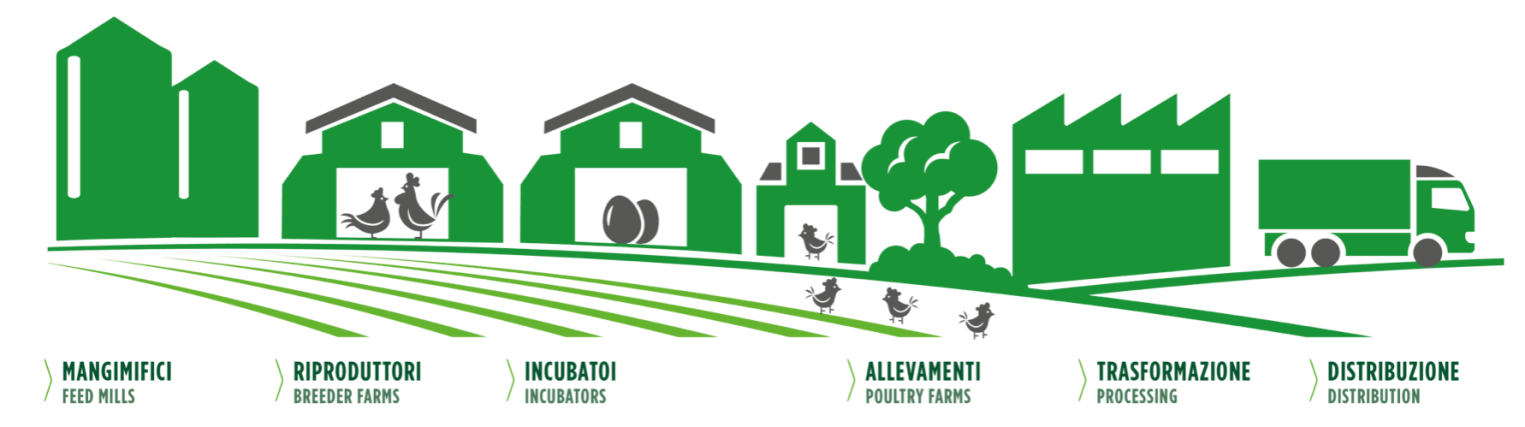
\includegraphics[width=0.95\textwidth]{figures/supplychain.png}
    \caption{The Vertically Integrated Supply Chain Architecture of Amadori S.p.A.}
    \label{fig:integrated_supply_chain}
\end{figure}

To operationalize complete transparency, Amadori enforces a comprehensive Traceability and Safety Governance framework. 
Digital tracking systems record every unit movement from raw feed batch origin to primary processing date, portioning line, and final distributor dispatch. 
This structural control protects brand equity, fulfills rigorous international certification standards, and guarantees total food safety compliance across all production hubs.

\section[Portfolio Strategy]{Multi-Protein Strategy and Manufacturing Complexity}
\label{sec:portfolio_strategy}

To address shifts in consumer demand, dietary habits, and retail channel dynamics, Amadori has expanded its commercial focus under a multi-protein strategy. 
The group has moved beyond its traditional poultry core into a multi-category product portfolio structured across four distinct protein sources:
\begin{itemize}
    \item \textbf{White Proteins (Poultry):} The core volume driver of the company, centered on integrated chicken and turkey operations.
    \item \textbf{Yellow Proteins (Eggs):} Shell egg production and liquid egg products designed for both direct retail sales and food service manufacturing.
    \item \textbf{Pink Proteins (Pork):} Fresh and cured pork charcuterie, expanded strategically through the acquisition of the \textit{Lenti} brand, 
    which specializes in high-end cooked hams and deli counter items.
    \item \textbf{Green Proteins (Plant-Based):} Alternative vegetable proteins derived from soy, pea, and cereal grains, 
    consolidated through the acquisition of the \textit{Unconventional} brand to capture market share within flexitarian and alternative food segments.
\end{itemize}

From a supply chain perspective, this diversified portfolio introduces substantial operational complexity. 
Managing multi-protein manufacturing lines requires strict segregation between meat and plant-based processing to prevent cross-contamination, 
separate production scheduling calendars, and domain-specific inventory management rules across fresh, cured, and frozen storage categories.

\section[Operational Constraints]{Operational Constraints: Biological Lead Times, Perishability, and Component Balancing}
\label{sec:operational_constraints}

The operational management of Amadori's poultry value chain is governed by three non-negotiable physical and biological constraints:
\begin{itemize}
    \item \textbf{Biological Inelasticity and Upstream Lead Times:} Unlike discrete manufacturing industries where raw material procurement can 
    scale dynamically to demand shocks, livestock production follows rigid biological timelines. Breeding, incubation, and grow-out cycles are structurally fixed; 
    an increase or decrease in downstream market demand cannot immediately alter the volume of birds already placed on farms weeks or months earlier. 
    Upstream production is therefore highly inelastic.
    \item \textbf{High Product Perishability:} Fresh and ultra-fresh poultry items have limited shelf lives, ranging from several days to a few weeks depending 
    on packaging technologies (e.g., modified atmosphere). This leaves virtually no room for inventory buffering: holding excess finished stock leads directly 
    to product obsolescence, mandatory price discounting, or physical scrap.
    \item \textbf{Anatomical Component Balancing:} A bird represents an indivisible biological unit that must be processed in its entirety. 
    Consumer and retail demand, however, is structurally asymmetrical: market demand frequently spikes for specific cuts (such as chicken breasts or thighs) 
    due to seasonal trends or retail promotions, while demand for remaining anatomical cuts (wings, legs, or carcasses) may remain flat or decline. 
    Operational planning must constantly balance these proportions, diverting surplus parts into frozen storage, secondary processing (frankfurters, breaded items), 
    or industrial food service to prevent costly structural imbalances.
\end{itemize}

\section[Demand Planning Rationale]{Strategic Rationale: Demand Planning as the Core Thesis Use Case}
\label{sec:demand_planning_rationale}

The convergence of biological supply inelasticity, extreme product perishability, and anatomical component balancing establishes the operational context of this thesis. 
In Amadori's business model, \textbf{Demand Planning represents the critical operational bridge} reconciling rigid agricultural production with volatile market demand.

Downstream retail demand is inherently unstable, driven by weekly promotions in modern supermarkets, weather fluctuations, and holiday calendars. 
Conversely, upstream farming schedules cannot be altered on short notice. In this environment, stochastic demand forecasting cannot be treated merely as a 
commercial exercise; it serves as the foundational steering mechanism for the entire Sales and Operations Planning cycle. Accurate demand signals determine 
line balancing schedules, guide procurement parameters, and stabilize logistics dispatches.

Underestimating demand leads to retail stockouts, service-level penalties from supermarket chains, and lost revenue. Overestimating demand generates stock 
surpluses that expire quickly, triggering distress discounts, unplanned cold-storage costs, and food waste. Furthermore, the downstream Material Planning 
engine—which calculates gross component requirements for packaging, labels, and ingredients as detailed in \Cref{chap:demandforecast}—is directly dependent 
on the accuracy and stability of this upstream demand forecast.

Because improving the speed, semantic clarity, and computational accessibility of these demand and material signals yields the highest operational impact for 
the enterprise, Demand Planning was selected as the foundational use case for this thesis.